\section{Model}
\subsection{Motivation}
This paper builds on the dynamic discrete choice framework by \cite{Agu2023}, in which consumer purchase behaviour is modelled as a dynamic decision problem with state dependence. In the framework, past purchase behaviour affects current choices through the duration since the last purchase. This is particularly relevant for storable goods such as canned tuna, where the timing of previous purchases contains information about the consumer’s current inventory. Other papers, such as \cite{HendelNevo2006}, model inventory more explicitly. However, in this paper, we model the duration since the last purchase as a proxy for consumers' inventory level. We will discuss this assumption later in Section 7. While the model is motivated by the framework of \cite{Agu2023}, we estimate it using the Nested Fixed Point (NFXP) algorithm developed by \cite{Rust1987} rather than the conditional maximum likelihood approach. 
\\
\\ 
In principle, Aguirregabiria’s estimator would be attractive because it controls for fixed-effects unobserved heterogeneity without solving the dynamic programming problem. However, the estimator relies on observing consumers with specific choice histories that visit the same states in different orders. In our empirical data, these identifying histories are rare, with only 153 eligible choice histories available. This leaves too little identifying variation to reliably estimate the conditional maximum likelihood model. We therefore estimate a simpler structural model using NFXP.

%Jeg har rettet ovenstående fra: 
%In our empirical data, these identifying histories are rare, where only 153 choice histories would be sufficient. This leaves too little identifying variation to reliably estimate the conditional maximum likelihood model. We therefore estimate a simpler structural model using NFXP. 



\subsection{Setup}
In the model, there are \textit{J} different brands of a storable good which are indexed as $j \in \{1,2...,J\}$. Consumers are indexed by  $i \in \{1,2...,N\}$ and time as $t \in \{1,2,...,T\}$. As in \cite{Agu2023}, we index time by weeks to also include weeks in which consumers have not purchased the storable good. However, we slightly modify the indexing of time in order to account for the retailer's promotional week \footnote{Netto's promotions run from Saturday to Friday. Therefore, when aggregating the data to the weekly level, we define a promotion week as running from Saturday to Friday rather than using the standard calendar week.}. In our empirical application, we use $J = 2$ (Glyngøre \& Navito) and $T = 52$ weeks. Both brands offer \textit{canned tuna in oil} and \textit{canned tuna in water} variants. We aggregate the two variants of each brand into a single product because the analysis focuses on brand choice rather than variant choice. Furthermore, the effect of choosing one variant over another cannot be estimated because promotions are symmetric across variants. 
\\
\\
In each period, \textit{t}, consumer \textit{i} chooses an action, $y_{it}$ from the following choice set
\begin{align}
   y_{it} \in\mathcal{Y} &= 0  \cup j \in \{1,2...,J\}
\end{align}
Where $y_{it} = 0$ denotes the no purchase option and $y_{it} = j$ denotes the brand choice that each consumer chooses, which yields $J+1$ different choice alternatives. 


\subsection{Utility Function}

We define the utility function by closely following \cite{Agu2023}, but without allowing for consumer-specific unobserved heterogeneity. Hence, brand preferences are assumed to be common across consumers. Consumer $i$'s per-period utility from action $y_{it}$ is given by
\begin{equation}
U_{it}(y_{it})
=
u(y_{it},x_{it},p_{it})
+
\varepsilon_{it}(y_{it}),
\end{equation}
where the deterministic part of the utility is specified as
\begin{equation}
u(y_{it},x_{it},p_{it})
=
\begin{cases} 
\alpha_{\ell_{it}}
-
\beta^{\text{dep}}(\ell_{it},d_{it})
& \text{if } y_{it}=0, \\[6pt]

\alpha_j
-
\gamma \cdot p_{it}(j)
-
\beta^{\text{sc}}(\ell_{it},j)
& \text{if } y_{it}=j
\end{cases}
\end{equation}
The state variables are later defined in section 2.7 and 2.8. 
\\
\\
In both the simulation and the empirical application of the model, one brand-specific constant is normalised for identification. We normalise the brand-specific constant for Glyngøre, $\alpha_1$, to zero. The parameter $\alpha_2$ should therefore be interpreted relative to Glyngøre. In the purchase utility, $\alpha_2$ captures the utility component of choosing Navito relative to Glyngøre, holding prices and switching costs fixed. However, because the no-purchase utility also depends on the previously purchased brand through $\alpha_{\ell_{it}}$, $\alpha_2$ also affects the utility of not purchasing when Navito was the last brand purchased. The parameter should therefore be interpreted as a relative brand-specific utility component rather than a pure brand preference parameter for current purchases alone. With this in mind, a negative value of $\alpha_2$ should be interpreted as consumers having a lower average preference for Navito compared to Glyngøre. Conversely, a positive value should be interpreted as consumers having a higher preference for Navito compared to Glyngøre. 

\subsection{Transition Rule}
We define the following transition rule by closely following \cite{Agu2023}
\[
(\ell_{i,t+1},d_{i,t+1})=
\begin{cases}
(\ell_{it},\,d_{it}+1) & \text{if } y_{it}=0,\\[2pt]
(j,\,1)                     & \text{if } y_{it}=j
\end{cases}
\]
With no purchase, $y_{it} = 0$, the brand state stays unchanged, $\ell_{it}=\ell_{i,t+1}$, while duration, $d$, increments by 1. In case of a purchase, the brand state is updated with $j_{it}=\ell_{i,t+1}$.



\subsection{Consumer Decision Problem} 
In each period, the consumer decides whether or not to purchase canned tuna. In each period \textit{t}, consumer \textit{i} observes the state, $s_t = (x_{t},\varepsilon_{t})$ where $x_t$ contains the state variables and $\varepsilon_t$ is the error term. The observed state variables are given as $x_t = (\ell_{it},d_{it},p_{it})$. The state variables are further described in section 2.7 and 2.8.  The action \(y\) corresponds to the consumer's choice \(y_{it}\), where \(y=0\) denotes no purchase and \(y=j\) denotes the purchase of brand \(j \in \{1,\ldots,J\}\). Hence, \(y \in \mathcal{Y}\).
\\
\\
Consumers maximise the discounted sum of the utilities. Following \cite{rust1994structural}, the consumer's problem can be represented as a Markov decision process, since current utility depends on the current state and action, and the transition of future states depends only on the current state and the action chosen in the current period. The consumers have a set of actions $y \in \mathcal{Y}$ where $\mathcal{Y} \in \{0,1,...,J\}$ that solves the following 
\begin{align*}
    V(s)
=
\max_{\delta}
\mathbb{E}_t
\left[
\sum_{t=0}^{\infty}
\beta^t
U(s_t,y_t)
\mid s_0=s
\right].
\end{align*}
Where $\beta \in (0,1)$ is the discount factor. In each period, the consumer observes the current state and chooses an action $y_{it}$. This action determines the consumer's current utility and also affects the state in the next period. For example, if the consumer does not purchase, the duration since last purchase increases, while a purchase updates the last brand purchased and resets the duration state. The evolution of the state follows a Markov Transition Probability, meaning that next period's state depends only on the current state and the current action, not on the full history of previous choices. This allows the optimal decision rule to be found recursively, given by the Bellman equation.
\begin{align*} 
    V(x,\varepsilon) =\max_{y \in \mathcal{Y}} \{ u_t(s_t,y) + \beta \mathbb{E}[V(x',\varepsilon')\vert x, \varepsilon,y]\} \tag{2.1}
\end{align*}
The notation \(x'\) and \(\varepsilon'\) denotes the next period's state and error term, so \(V(x',\varepsilon')\) is the future value the consumer expects after making the current decision.
\\
\\
After formulating the Bellman equation, the next step is to explicitly express the expectation over future states. Since the consumer does not know the next period’s state and utility shocks with certainty, the expected value function is evaluated by integrating over all possible future states and shocks
\begin{align*}
    \mathbb{E}[V(x',\varepsilon') \vert x,\varepsilon,y)] = \int_X \int_\Omega V(x',\varepsilon') p(x',\varepsilon' \vert x,\varepsilon,y)dx'd\varepsilon' \tag{2.2} 
\end{align*}
Following \cite{Rust1987} the above dynamic discrete choice problem can be simplified by imposing three key assumptions. 
\begin{quote}
\paragraph{Assumption 1:} Utility is assumed to be additively separable in preferences, $U_t(s_t,y) = u(x_t,y,\theta) + \varepsilon_t(y)$. The parameter vector $\theta $ contains the utility parameters that determine how observed states and choices affect current utility. The additive separability assumption implies that unobserved factors enter utility only through the choice-specific shock and do not interact directly with the observed state variables.
\end{quote}
\begin{quote}
\paragraph{Assumption 2:} The model assumes conditional independence. Conditional on the current observed state, $x_t$, and choice $y_t$, the next observed state, $x_{t+1}$ evolves independently from $\varepsilon_t$ which formally can be written as 
\begin{align*}
    p(x_{t+1}, \varepsilon_{t+1} \vert x_t,\varepsilon_t,y) = q(\varepsilon_{t+1} \vert x_{t+1}) p(x_{t+1} \vert x_t,y)
\end{align*}
In this paper, this implies that once the consumer’s current purchase decision is observed, the evolution of duration since last purchase depends on the current state and decision, but not directly on the current utility shock.
\end{quote}
\begin{quote}
\paragraph{Assumption 3:} The choice-specific shocks are assumed to be independently and identically distributed Type I extreme value.
\end{quote}
\\
\\ 
Using \textbf{Assumption 1}, the per-period utility can be written as the sum of a deterministic component and a choice-specific shock, $U(x,y,\varepsilon) = u(x,y) + \varepsilon(y).$
Using\textbf{ Assumption 2}, the transition of next period's observed state is conditionally independent of the current utility shock once the current state and action are given. Hence, the distribution of next period's observed state and utility shock can be factorized as $p(x',\varepsilon' \mid x,\varepsilon,y) = p(x' \mid x,y)q(\varepsilon' \mid x')$. Therefore, the Bellman equation can be written as follows
\begin{align*}
     V(x,\varepsilon) = \max_{y \in \mathcal{Y}} \{u(x,y) + \varepsilon(y) + \beta \int_X \int_{\Omega} V(x',\varepsilon')p(x' \vert x,y)q(\varepsilon' \vert x')dx'd\varepsilon'\}
\end{align*} 
Because of \textbf{Assumption 2}, conditional independence implies that, once the current observed state $x$ and action $y$ are given, the distribution of next period's observed state $x'$ does not depend directly on the current utility shock $\varepsilon$. Hence, the consumer only needs to form expectations over the possible next-period observed states and next-period utility shocks.\\
\vspace{-1cm}
\begin{align*}
    EV(x,y) 
    &= \Gamma(EV)(x,y) \\
    &= \int_{X} \int_{\Omega} 
    V(x',\varepsilon')
    p(x' \mid x,y)
    q(\varepsilon' \mid x')
    \, d\varepsilon' \, dx' .
\end{align*} 
Here, \(EV(x,y)\) is the expected value of future utility after choosing action \(y\) in state \(x\). The future value function is given by
\begin{align*}
    V(x',\varepsilon') 
    =
    \max_{y' \in \mathcal{Y}}
    \left\{
    u(x',y') + \beta EV(x',y') + \varepsilon'(y')
    \right\}.
\end{align*}
\noindent
The difficulty is that $V(x',\varepsilon')$ contains the maximum over all future choices. Without further assumptions, evaluating this expectation would require integrating over the full vector of future shocks. \textbf{Assumption 3} solves this problem by assuming that the choice-specific shocks are independently and identically Type I extreme value distributed. Under this assumption, the expectation of the maximum has a closed-form log-sum representation
\begin{align*}
    \int_{\Omega}
    V(x',\varepsilon')
    q(\varepsilon' \mid x')
    d\varepsilon'
    =
    \log
    \left[
    \sum_{y' \in \mathcal{Y}}
    \exp
    \left(
    u(x',y')
    +
    \beta EV(x',y')
    \right)
    \right].
\end{align*}
Substituting this expression into the expected value function gives
\begin{align*}
    EV(x,y)
    =
    \Gamma(EV)(x,y)
    =
    \int_X
    \log
    \left[
    \sum_{y' \in \mathcal{Y}}
    \exp
    \left(
    u(x',y')
    +
    \beta EV(x',y')
    \right)
    \right]
    p(x' \mid x,y)
    dx'.
\end{align*}
This implies that the conditional choice probabilities (CCP) can be written in closed-form logit form
\begin{align*}
    P(y \mid x)
    =
    \frac{
    \exp
    \left[
    u(x,y)
    +
    \beta EV(x,y)
    \right]
    }{
    \sum_{y  \in \mathcal{Y}}  
    \exp
    \left[
    u(x,a)
    +
    \beta EV(x,a)
    \right] \tag{2.3}
    }.
\end{align*}
The numerator represents the exponentiated value of choosing action $y$ in state $x$, while the denominator sums the corresponding value across all actions (denoted as $a$ in 2.3) . Hence, the probability of choosing $y$ depends on both current utility and the expected value function. 

\subsection{Estimation using the Nested Fixed Point Algorithm}

The model is estimated by maximum likelihood using the Nested Fixed Point (NFXP) algorithm developed by \cite{Rust1987}. The key challenge is that the CCP depend on the expected value function, and the expected value function itself depends on the structural parameters. Therefore, the likelihood cannot be evaluated from current-period utility alone.
\\
Let $\theta$ denote the vector of structural parameters. We write $\theta=(\theta_u,\theta_p)$, where $\theta_u$ contains the utility parameters and $\theta_p$ contains the parameters governing the transition process of the state variables. For a given parameter vector $\theta$, the expected value function satisfies the fixed point equation
\begin{align*}
EV_\theta(x,y)
=
\Gamma_\theta(EV_\theta)(x,y),
\end{align*}
where $y \in \mathcal{Y}$ denotes the current action. 
\\
\\
Given the Type I extreme value assumption, the model implies closed-form conditional choice probabilities. For a consumer in state $x$, the probability of choosing action $y$ is
\begin{align*}
P_\theta(y \mid x)
=
\frac{
\exp\left[
u(x,y,\theta_u)+\beta EV_\theta(x,y)
\right]
}{
\sum_{a\in\mathcal{Y}}
\exp\left[
u(x,j,\theta_u)+\beta EV_\theta(x,j)
\right]
}.
\end{align*}
The NFXP algorithm estimates the model using two nested loops. In the \textit{inner loop}, the expected value function is solved for a given parameter vector, $\theta$. This is done by iterating on the fixed point equation $EV_\theta = \Gamma_\theta(EV_\theta)$
until convergence. Since the discount factor satisfies $\beta \in (0,1)$, the Bellman operator is a contraction mapping. This implies that the fixed point is unique and that value function iteration converges to a unique solution.
\\
In the \textit{outer loop}, the parameter vector is updated in order to maximize the likelihood of the observed choices. Given a parameter vector $\theta$, the inner loop first solves for $EV_\theta$. The resulting expected value function is then used to compute the conditional choice probabilities $P_\theta(y_{it}\mid x_{it})$. The choice log-likelihood is therefore given by
\begin{align*}
    \ell(\theta)
=
\sum_{i=1}^{N}
\sum_{t=1}^{T_i}
\log P_\theta(y_{it}\mid x_{it})
\end{align*}
where $y_{it}$ is the observed choice of consumer \textit{i} in period \textit{t}, and $x_{it}$ is the corresponding observed state. The outer-loop maximazation problem can then be written as
\begin{align*}
\hat{\theta}
=
\arg\max_{\theta}
\ell(\theta).
\end{align*}
Thus, the estimated parameters are the values of $\theta$ that make the observed sequence of consumer choices most likely, given the expected value function solved in the inner loop. The \textit{outer loop} maximization is carried out using the BFGS algorithm.  

\newpage
\subsection{Price Process}
Prices enter the model through a weekly promotion process. Since the empirical model is estimated at the weekly level, we assume that consumers observe the current price of each brand at the beginning of each period. For each brand \textit{j}, the price in week \textit{j} depends on whether the brand is on promotion. We let $e_t = (e_{1t},e_{2t})$ where $e_{jt} = 1$ if brand $j$ is promoted in week $t$ and $e_{jt} = 0$ otherwise. 
This implies that prices enter the utility function in the following way
\begin{align*}
    p_t(j) =
    \begin{cases}
        p_j^{RRP} & \text{if } e_{jt} = 0 \\
        p_j^{PP} & \text{if } e_{jt} = 1
    \end{cases}
\end{align*}
Where $p_j^{RRP}$ is the recommended retail price and $p_j^{PP}$ is the promotional price. Equivalently, the price can be written as
\begin{align*}
    p_t(j) = p_j^{RRP} - \Delta_j e_{jt}
\end{align*}
Where $\Delta_j = p_j^{RRP} - p_j^{PP}$ denotes the promotional discount. 
In a static model, consumers would respond only to the prices observed in the current period. In the present framework, however, consumers are forward-looking and may therefore also take expected future prices into account when making their current purchase decision. This is particularly relevant for storable goods such as canned tuna, where consumers can shift purchases across time. If a consumer expects that a brand may be promoted in a future week, it may be optimal to postpone the purchase. Conversely, if the current price is low due to a promotion, purchasing today may be attractive because the consumer can store the product and reduce the need to buy in future periods. In the empirical application, the transition matrix for the promotion process is estimated from the observed weekly promotion patterns in the data. The transition matrix summarises how likely each promotion state is to be followed by another promotion state in the next period. Once estimated, the transition matrix is treated as known when solving the consumer's dynamic programming problem. This allows consumers in the model to form expectations about future promotion states based on the observed promotion process. At the same time, promotions are assumed to be exogenous from the perspective of the individual consumer. That is, consumers take the retailer's current and future pricing process as given, and an individual consumer's purchase decision does not affect the retailer's future promotion decisions.

\subsection{Interpretation of Switching Costs and Depletion}
Two central parameters in the model are the switching costs parameter, $\beta^{sc}$ and the depletion parameter, $\beta^{dep}$. These parameters capture two forms of state dependence. The switching cost parameter captures persistence in brand choice. The depletion parameter captures how purchase propensity varies with time since the last purchase.
\begin{align*}
    \beta^{sc} \mathbb{I} \{\ell_{it} \neq j\}
\end{align*}
The switching cost parameter enters the utility of purchasing brand $j$ when the brand differs from the previously purchased brand, $\ell_{it}$. If $\beta^{sc} > 0$, switching away from the previously purchased brand lowers current utility, since the term enters the utility function with a negative sign (see section 2.3). This behaviour generates brand persistence. If positive, $\beta^{sc} > 0$, consumers are more likely to choose the same brand as previously. Larger values of $\beta^{sc}$ therefore implies stronger brand loyalty, habit formation or search costs. The switching costs parameter is motivated by the literature on brand persistence and consumer brand inertia. Empirically, \cite{article} shows substantial persistence in brand choice by households in consumer goods. 
\\
\\
The depletion parameter, $\beta^{dep}$, captures the role of duration since last purchase. Hence, if consumers chooses the no purchase option, the utility is the following 
\begin{align*}
    u_{it}(0,x_{it},p_{it}) = \alpha_{it} - \beta^{dep}
\end{align*} 
If $\beta^{dep} > 0$, an increase in duration, $d$, is associated with higher log-odds of purchasing, ceteris paribus. The intuition behind this is that the longer it has been since the previous purchase, the more likely the consumer's inventory is to be depleted and therefore to restock. If $\beta^{dep}<0$, the model instead implies that longer duration is associated with a lower probability of purchase, which might seem counterintuitive. It should be noted that we restrict the duration since last purchase to be capped at 25 weeks. This implies that all durations of 25 weeks or more are assigned the same terminal duration state (25+ weeks). We impose this restriction in order to reduce the state space.  
\\
\\
It should be noted that we, in both the simulation and empirical application of the model, assume both symmetric switching costs and depletion parameters. Hence, we impose the following restrictions:
\begin{align*}
    \beta^{dep}_1 &= \beta^{dep}_2 = \beta^{dep} \\
    \beta^{sc}_{12} &= \beta^{sc}_{21} = \beta^{sc}
\end{align*}
We introduce these restrictions to simplify the model and reduce the computational burden. A common depletion parameter implies that the duration since the last purchase affects the probability of purchasing in the same way, regardless of which brand was previously purchased. We argue that this is plausible since both brands of canned tuna carry the same size can. Similarly, a common switching cost parameter implies that switching from Glyngøre to Navito has the same utility cost as switching from Navito to Glyngøre.  



\subsection{Initial Conditions Problem}
A common challenge in dynamic discrete choice models is the initial-conditions problem. Our model contains lagged state variables: the last brand purchased and the duration since the last purchase. Since consumers' pre-sample purchase histories are not observed, the values of these states at the beginning of the empirical sample are unknown. A classic discussion is provided by \cite{NBERc8909}: if the initial states are correlated with persistent unobserved heterogeneity, ignoring this dependence can bias the parameter estimates.
\\
\\
We handle the initialization of the lagged state variables differently in the Monte Carlo simulation and the empirical application. In the Monte Carlo simulation, we generate a number of pre-sample weeks and discard them before estimation. During this burn-in period, consumers make simulated choices and the endogenous state variables evolve according to the model's transition rules. Consequently, the recorded sample is less dependent on the arbitrary state values assigned at the start of the simulation and more closely reflects the model-implied distribution of consumer histories.
\\
\\
This approach is not possible in the empirical application because consumers' pre-sample purchase histories are unobserved. We therefore exclude observations up to and including each consumer's first observed purchase from the likelihood. The first observed purchase is used to initialize the last-brand and duration states, and estimation is based on subsequent observations. This approach has its limitations. First, it reduces the sample size. This is particularly relevant in our data set because consumers have a minimum of only five purchases and the sample covers only one year. Second, the model does not explain each consumer's first observed purchase. Finally, this trimming rule does not fully solve the initial-conditions problem if the state variables remain correlated with persistent unobserved heterogeneity.

%Old version: A common challenge in (dynamic) discrete choice models is the initial conditions problem. The model contains lagged state variables, which in this case are the last brand purchased and the duration since last purchase. We assume that these states affect current consumer choice. However, at the beginning of the sample period, we did not observe the consumers' pre-sample history. Therefore, the first observed state may not correspond to the consumer's true initial state. This issue was first discussed by \cite{NBERc8909}, where the initial states may be correlated with unobserved heterogeneity. This can lead to bias in the parameter. We control for the initial states in both the simulation and the empirical application. In the Monte Carlo simulation we can control the environment and thus control for the initial states by adding a burn-in period to the true DGP. As this is not possible in a natural environment, like our empirical data, we handle this by excluding each consumer's first observed purchase from the maximum likelihood, and instead use the first observed purchase to initialise the last brand purchased. However, this approach is expectedly prone to limitations. First, it reduces the sample size because consumer's first purchase is excluded from the likelihood. This is particularly significant in our data set since consumers only has a minimum of five purchases and the data set only contains data for one year. Second, the model does not explain the consumer's first observed purchase. 





\newpage
\section{Monte Carlo Simulation}

The purpose of the Monte Carlo simulation is to evaluate whether the NFXP estimator can recover the structural parameters of the dynamic demand model in a controlled setting. In the empirical application, the true parameters are unobserved. It is therefore difficult to know whether an estimated parameter reflects the underlying economic mechanism, numerical features of the estimator or misspecification of the model. The Monte Carlo exercise addresses this issue by generating simulated data from the model with known parameters and then re-estimating the model on the simulated data.

\subsection{Data-generating process}

The Monte Carlo exercise is based on a data-generating process (DGP). A DGP is a fully specified artificial environment that describes how the data would be generated if the model were the true description of consumer behaviour. The DGP therefore specifies preferences, prices, the promotion process, state transitions and the distribution of the choice-specific shocks.
\\
\\
The simulation proceeds as follows. First, we specify the model environment by fixing the true parameter values, prices, promotion process, state space and discount factor. Second, the dynamic programming problem is solved at the true parameter vector, yielding the value function and the conditional choice probabilities. Third, a panel of artificial consumers is generated by drawing choices from these probabilities. The simulated panel, therefore, contains the same objects as the empirical data: weekly choices, last-purchased brand, duration since last purchase, and promotion states.
\\
\\
The key advantage is that the true parameter vector is known by construction. If the estimator performs well under the correctly specified DGP, the estimates should be close to the true values across repeated simulated samples. If the estimator fails in this setting, this would indicate either numerical problems or weak identification before the model is taken to real data.

\subsection{Calibration and simulation design}

The Monte Carlo calibration chooses numerical values for the primitives of the DGP. The calibration uses the same choice set, state variables and dynamic structure as the empirical model, but fixes the structural parameters at known values. In the baseline simulation, the true parameter vector is
\[
\theta_0
=
\left(
\alpha_2,\gamma,\beta^{\text{sc}},\beta^{\text{dep}}
\right)
=
\left(
0.50,\;0.05,\;0.40,\;0.275
\right),
\]
with $\alpha_1$ normalized to zero.
\\
\\
Prices follow the hi-lo promotion process described above, with regular prices, promotional discounts and promotion probabilities fixed before simulation. The discount factor is fixed at $0.95$, and the duration state is capped at $D_{\max}=25$ in the numerical implementation.

% [Insert Table MC1, Panel A here: calibrated DGP primitives]
\begin{table}[H]
\centering
\caption{Monte Carlo DGP Inputs}
\label{tab:mc_dgp_primitives}
\begin{tabular}{ll}
\toprule
DGP input & Calibration \\
\midrule
Brands, $J$ & 2 \\
Discount factor & 0.95 \\
Duration cap, $D_{\max}$ & 25 \\
True parameters $(\alpha_2,\gamma,\beta^{sc},\beta^{dep})$ & (0.500, 0.050, 0.400, 0.275) \\
Regular prices, $(p^0_1,p^0_2)$ & (11.95, 24.95) \\
Promotional discounts, $(\Delta p_1,\Delta p_2)$ & (1.95, 15.67) \\
Promotion entry probabilities & (0.192, 0.115) \\
Promotion persistence & 0.000 \\
\bottomrule
\end{tabular}
\end{table}

\noindent
The simulated panel contains $N=50{,}000$ consumers observed for $T=52$ weeks, after a burn-in period of 104 weeks. The baseline exercise uses $R=50$ Monte Carlo replications, and the NFXP estimator is initialised from several starting values in each replication.

% [Insert Table MC1, Panel B here: simulation and estimation design]
\begin{table}[H]
\centering
\caption{Monte Carlo simulation and estimation design}
\label{tab:mc_sim_design}
\begin{tabular}{ll}
\toprule
Simulation parameters & Value \\
\midrule
Consumers per panel, $N$ & 50,000 \\
Weeks per consumer, $T$ & 52 \\
Burn-in weeks & 104 \\
Monte Carlo replications, $R$ & 50 \\
NFXP starts per replication & 3 \\
Default starting value & (0.250, 0.040, 0.250, 0.200) \\
\bottomrule
\end{tabular}
\end{table}

\subsection{Estimation and Monte Carlo statistics}

For each simulated panel, the model is re-estimated by maximum likelihood using the same NFXP procedure as in the empirical application. The inner loop solves the dynamic programming problem for each trial value of $\theta$, while the outer loop chooses the parameter vector that maximises the simulated choice likelihood
\[
\ell_r(\theta)
=
\sum_{i=1}^{N}
\sum_{t=1}^{T}
\log P_{\theta}(y_{it}^{r}\mid x_{it}^{r}),
\]
where $r$ indexes the Monte Carlo replication. The promotion process is treated as known, so the estimated likelihood is based on the choice probabilities. For each replication, the solution with the highest likelihood across the starting values is retained.
\\
\\
For each parameter $\theta_k$, parameter recovery is summarized by the mean estimate, bias and root mean squared error:
\[
\overline{\hat{\theta}}_k
=
\frac{1}{R}\sum_{r=1}^{R}\hat{\theta}_{rk},
\qquad
\text{Bias}_k
=
\overline{\hat{\theta}}_k-\theta_{0k},
\]
and
\[
\text{RMSE}_k
=
\left[
\frac{1}{R}
\sum_{r=1}^{R}
\left(\hat{\theta}_{rk}-\theta_{0k}\right)^2
\right]^{1/2}.
\]

% [Insert Table MC2 here: Monte Carlo parameter recovery]
\begin{table}[H]
\centering
\small
\caption{Monte Carlo parameter recovery}
\label{tab:mc_parameter_recovery}
\begin{tabular}{lrrrrrr}
\toprule
Parameter & True & Mean est. & Bias & Rel. bias (\%) & Std. dev. & RMSE \\
\midrule
$\alpha_2$ & 0.500 & 0.4998 & -0.0002 & -0.05 & 0.0012 & 0.0012 \\
$\gamma$ & 0.050 & 0.0500 & -0.0000 & -0.07 & 0.0001 & 0.0001\\
$\beta^{sc}$ & 0.400 & 0.4005 & +0.0005 & +0.14 & 0.0018 & 0.0019 \\
$\beta^{dep}$ & 0.275 & 0.2748 & -0.0002 & -0.08 & 0.0010 & 0.0010 \\
\bottomrule
\end{tabular}
\vspace{-0.5cm}
\begin{flushleft}
\end{flushleft}
\end{table}

% [Insert Figure MC1 here: distribution of Monte Carlo estimates relative to true values]
\begin{figure}[H]
    \centering
    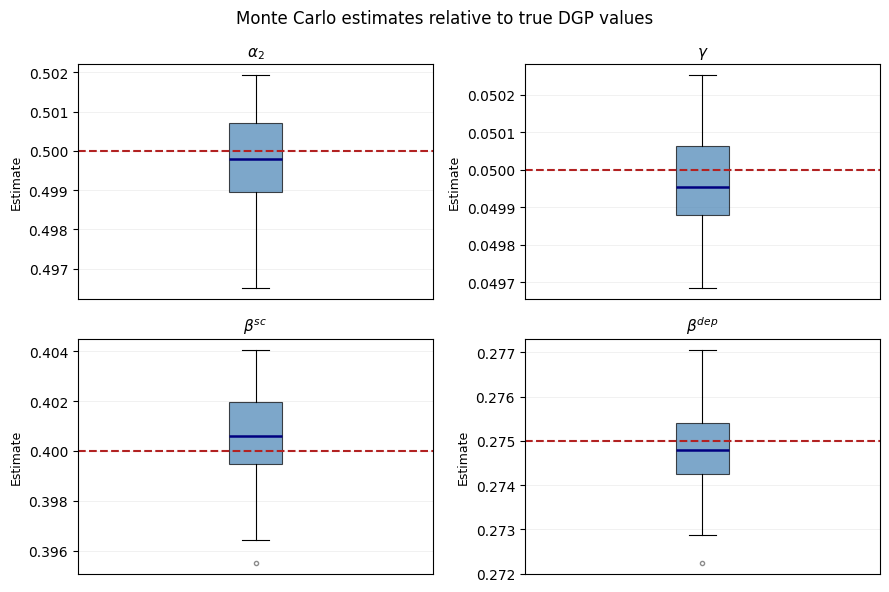
\includegraphics[width=0.85\linewidth]{nfxp_mc_boxplots_original.png}
    \caption{Distribution of Monte Carlo estimates.}
    \label{fig:mc_estimate_distribution}
\end{figure}
\noindent
% [Insert Table MC3 or Figure MC2 here: selected observed versus predicted simulated moments]

\subsection{Interpretation}

Under the correctly specified DGP, the NFXP estimator should recover the true parameter vector up to simulation error. In particular, the average estimates should be close to $\theta_0$, the bias and RMSE should be small relative to the true parameter values and the optimizer should converge reliably across replications. Failure to recover the true parameters in this controlled setting would indicate either numerical problems in the dynamic programming or likelihood routines, or weak identification of one or more structural parameters.
\\
\\
The above table reports the Monte Carlo parameter results. Overall, the estimator recovers the true parameters very accurately. The estimates are close to the true parameter values for all four parameters, and the biases are close to zero. For example, the true value og $\alpha_2$ is 0.50, while the mean estimate is 0.4998. The standard deviations and RMSE values are also small. This suggests that under the DGP process, the estimator is numerically stable and able to recover the underlying true parameters. The Monte Carlo simulation, therefore, provides evidence that the estimation procedure is correctly implemented before the model is applied to the scanner data. 

